\documentclass[conference]{IEEEtran}
\IEEEoverridecommandlockouts
\usepackage{cite}
\usepackage{amsmath,amssymb,amsfonts}
\usepackage{graphicx}
\usepackage{booktabs}
\usepackage{multirow}
\usepackage{xcolor}
\usepackage{tikz}
\usetikzlibrary{positioning,arrows.meta,fit,backgrounds}
\usepackage[hidelinks]{hyperref}
\usepackage{url}
\def\BibTeX{{\rm B\kern-.05em{\sc i\kern-.025em b}\kern-.08em T\kern-.1667em\lower.7ex\hbox{E}\kern-.125emX}}
\setlength{\textfloatsep}{6pt plus 2pt minus 2pt}
\setlength{\floatsep}{5pt plus 2pt minus 2pt}
\setlength{\dbltextfloatsep}{6pt plus 2pt minus 2pt}
\setlength{\abovecaptionskip}{2pt}
\setlength{\belowcaptionskip}{0pt}

\begin{document}

\title{UDI 2.0: A Verifiable Autonomous Data Analyst for Business Decision Intelligence on Heterogeneous Tabular Data}

\author{\IEEEauthorblockN{Deepanshul \quad Samarth Kamat}
\IEEEauthorblockA{Goa Institute of Management, Big Data Analytics\\
Roll No: B2026072, B2026098\\
Email: deepanshul2026b@gim.ac.in, samarth.kamat2026b@gim.ac.in}}

\maketitle

\begin{abstract}
Managers hold operational data but rarely have an analyst at hand to ask ``which country sells most?'', ``why did profit fall?'' or ``who is likely to leave?''. We present UDI~2.0, a conversational platform that answers such questions on any uploaded CSV/Excel table and turns the answers into business decisions. A planner (Gemini, or a trained offline intent model) converts each question into a structured plan; a validation gate checks every column, filter and data-sufficiency requirement against the real data; one of 18 controlled Python operations computes the result; and analyst, machine-learning and report agents add column-relationship maps, a 0--100 data-quality score with auto-cleaning, AutoML with one-standard-error model selection and SHAP explanations, forecasting with ARIMA/ETS candidates, root-cause decomposition and function-specific reports (sales, marketing, HR, operations, finance). On 104 held-out natural-language questions over four public and two generated datasets the offline planner reached 97.1\% intent accuracy and 88.5\% end-to-end correctness (96.2\% after fixing the defects that run exposed); numeric answers were checked against independent pandas oracles. On the public IBM HR, IBM Telco, UCI Bank Marketing and Global Superstore datasets the engine selected models with held-out ROC-AUC of 0.80--0.94, and the quality engine recovered 100\% of five injected defect types. All 168 automated tests pass.
\end{abstract}

\begin{IEEEkeywords}
Conversational analytics, AutoML, explainable AI, SHAP, data quality, decision intelligence, multi-agent systems
\end{IEEEkeywords}

\section{Introduction}
Business users in sales, marketing, HR and operations depend on analysts to translate questions into queries, models and charts. Dashboards answer only the questions they were built for, and large language models (LLMs) asked directly for numbers can hallucinate them~\cite{hong2024,tang2025}. Phase~1 of this project (UDI) showed that separating \emph{language interpretation} (Gemini planning) from \emph{numerical computation} (validated Python operations) prevents silent column substitution and invented numbers. Its review (20.2/30) identified four gaps that frame this paper: (i) no evaluation of routing and numerical correctness on held-out questions, (ii) no real-world datasets, (iii) results that stopped at analytics instead of decisions, and (iv) imprecise disclosure and test reporting.

\textbf{Business problem.} A manager should be able to upload a table and obtain, in minutes and without code, (a) correct answers with charts, (b) a clear picture of how the columns relate, (c) a trustworthy view of data quality, and (d) explained, quantified findings for a business function, while every number remains traceable to the data.

\textbf{Contributions.} (1) A hybrid planner: Gemini when available, otherwise a trained offline intent model with schema linking, both behind one validation gate. (2) A data-intelligence layer: business semantics per column, a mixed-type relationship map (associations, hierarchies, derived formulas, date rules) and a quality score with auditable cleaning. (3) Explainable AutoML: cross-validated selection with the one-standard-error rule, tuning, learning curves, time-ordered validation, leakage screening and exact-additivity SHAP. (4) Decision intelligence: root-cause decomposition, segmentation, forecasting with statistical baselines and a four-agent report pipeline with evidence-backed recommendations and PDF/Excel export. (5) A reproducible evaluation: a held-out question benchmark with oracles and pass/fail logs, four public datasets, a defect-injection study and an executed test report.

\section{Related Work}
Text-to-SQL and LLM data agents translate questions into executable actions~\cite{hong2024,tang2025,sun2024}. Data-Copilot~\cite{zhang2023} and LAMBDA~\cite{lambda2024} use predefined interfaces or cooperating agents; Data Interpreter~\cite{hong2024di} and AutoML-GPT~\cite{zhangautoml} let LLMs drive data-science pipelines; AGQS~\cite{saha2024} adds plan verification; AgenticData~\cite{sun2025agentic} and SageCopilot~\cite{liao2026} extend agentic analytics to reporting. Tool use is studied in Toolformer~\cite{schick2023} and ReAct~\cite{yao2022}. Unlike systems in which the LLM writes and runs code, UDI restricts execution to 18 validated operations, never lets a model produce a number, and adds a non-LLM fallback planner so the same guarantees hold offline. On the ML side we build on SHAP~\cite{lundberg2017} with the permutation estimator of~\cite{strumbelj2014}, the one-standard-error rule~\cite{hastie2009}, Isolation Forest~\cite{liu2008}, robust outlier scores~\cite{iglewicz1993}, bias-corrected Cram\'er's V~\cite{bergsma2013}, data-quality dimensions~\cite{wang1996} and forecasting practice with rolling-origin evaluation~\cite{hyndman2021}.

\section{System Architecture and Methodology}
\begin{figure}[t]
\centering
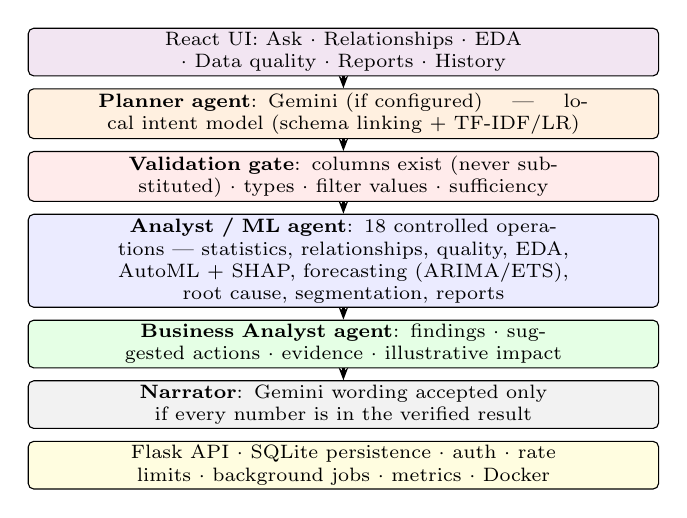
\begin{tikzpicture}[node distance=1.5mm, every node/.style={font=\scriptsize}, box/.style={draw, rounded corners=2pt, fill=#1, text width=7.9cm, minimum height=4.4mm, align=center, inner sep=1.5pt}, arr/.style={-{Stealth[length=1.6mm]}, thick}]
\node[box=violet!10] (ui) {React UI: Ask $\cdot$ Relationships $\cdot$ EDA $\cdot$ Data quality $\cdot$ Reports $\cdot$ History};
\node[box=orange!12, below=of ui] (pl) {\textbf{Planner agent}: Gemini (if configured) \quad | \quad local intent model (schema linking + TF-IDF/LR)};
\node[box=red!8, below=of pl] (vg) {\textbf{Validation gate}: columns exist (never substituted) $\cdot$ types $\cdot$ filter values $\cdot$ sufficiency};
\node[box=blue!8, below=of vg, minimum height=8.6mm] (ex) {\textbf{Analyst / ML agent}: 18 controlled operations --- statistics, relationships, quality, EDA,\\ AutoML + SHAP, forecasting (ARIMA/ETS), root cause, segmentation, reports};
\node[box=green!10, below=of ex] (ba) {\textbf{Business Analyst agent}: findings $\cdot$ suggested actions $\cdot$ evidence $\cdot$ illustrative impact};
\node[box=gray!10, below=of ba] (na) {\textbf{Narrator}: Gemini wording accepted only if every number is in the verified result};
\node[box=yellow!12, below=of na] (st) {Flask API $\cdot$ SQLite persistence $\cdot$ auth $\cdot$ rate limits $\cdot$ background jobs $\cdot$ metrics $\cdot$ Docker};
\foreach \a/\b in {ui/pl,pl/vg,vg/ex,ex/ba,ba/na} \draw[arr] (\a) -- (\b);
\end{tikzpicture}
\caption{UDI 2.0 runtime pipeline. Language models interpret and word; only Python computes.}
\label{fig:arch}
\end{figure}

\subsection{Planning: Gemini or an offline intent model}
Fig.~\ref{fig:arch} shows the pipeline. In \emph{auto} mode Gemini plans when an API key is configured; otherwise, or when a call fails, the local planner is used (\emph{gemini} and \emph{local} modes are strict). Gemini receives only the schema, column statistics, semantic types, a relationship digest and at most three sample rows, never the dataset. The local planner (i)~links n-grams to columns (exact, token, light inflection, curated same-concept synonyms, fuzzy match) and to category values, (ii)~masks them (\textit{``which catcol has the highest numcol''}), (iii)~classifies the masked question into 18 operations plus \emph{unsupported} with TF-IDF word (1--3) and character (2--5) n-grams and multinomial logistic regression trained on 1,658 templated questions, and (iv)~fills slots (target, grouping, aggregation, filters, horizon, scenario changes) deterministically. Because the intent model sees masked tokens, it generalises across schemas. A prediction with $\max_c P(c\mid q)<0.30$ becomes a clarification. A variable that is not a column is passed on verbatim, so the gate rejects it with the available columns.

\subsection{Validation gate and controlled operations}
Every plan is checked against the data before execution: column existence (only case/spacing variants are canonicalised), type compatibility, filter values present in the data, and operation-specific sufficiency (e.g.\ $\geq$24 periods to forecast, $\geq$5 rows per class). The ten Phase~1 operations are extended with \emph{query\_records}, \emph{pivot\_table}, \emph{run\_eda}, \emph{assess\_data\_quality}, \emph{describe\_relationships}, \emph{explain\_change}, \emph{segment\_records} and \emph{generate\_report}. ``Which country has the highest sales'' becomes \emph{compare\_groups} with $\Sigma$Sales by Country because Sales is semantically an additive money measure, whereas prices, rates and scores are averaged.

\subsection{Data intelligence: semantics, relationships and quality}
Each column receives a business semantic type (money, quantity, rate, score, duration, geography, product, outcome, flag, \dots) from name tokens and values. Pairwise association is measured on a common $[0,1]$ scale: $|r|$ (Pearson, or Spearman when clearly monotone-nonlinear) for numeric pairs, the correlation ratio $\eta=\sqrt{SS_B/SS_T}$ for numeric--categorical pairs, and bias-corrected Cram\'er's V~\cite{bergsma2013} for categorical pairs. Hierarchies $A\!\to\!B$ are reported when $\geq$98\% of the repeated values of the finer column map to one parent; derived columns $y=a\circ b$ ($\circ\in\{+,-,\times,\div\}$) when the identity holds within 1\% on $\geq$97\% of rows; date-ordering rules and candidate keys complete the data dictionary. The quality score combines five dimensions $d$ with measured defect rates $r_d$:
\begin{equation}
Q=\sum_{d} w_d\,100\left(1-\min(1,k_d r_d)\right),
\end{equation}
with $w=(.30,.20,.20,.15,.15)$ and $k=(1,4,4,4,2)$ for completeness (mean of missing-cell and incomplete-row rates), uniqueness, validity (unparsable values, impossible negatives, rates outside range), consistency (label variants, violated formulas and date rules) and outliers (modified $z>3.5$~\cite{iglewicz1993} \emph{and} beyond $3\times$IQR). Every issue carries a treatment (e.g.\ median imputation for a skewed variable, ``Unknown'' for categorical gaps, dropping columns $>$60\% missing); cleaning applies only selected actions, logs each change, reports before/after and is reversible.

\begin{figure}[t]
\centering
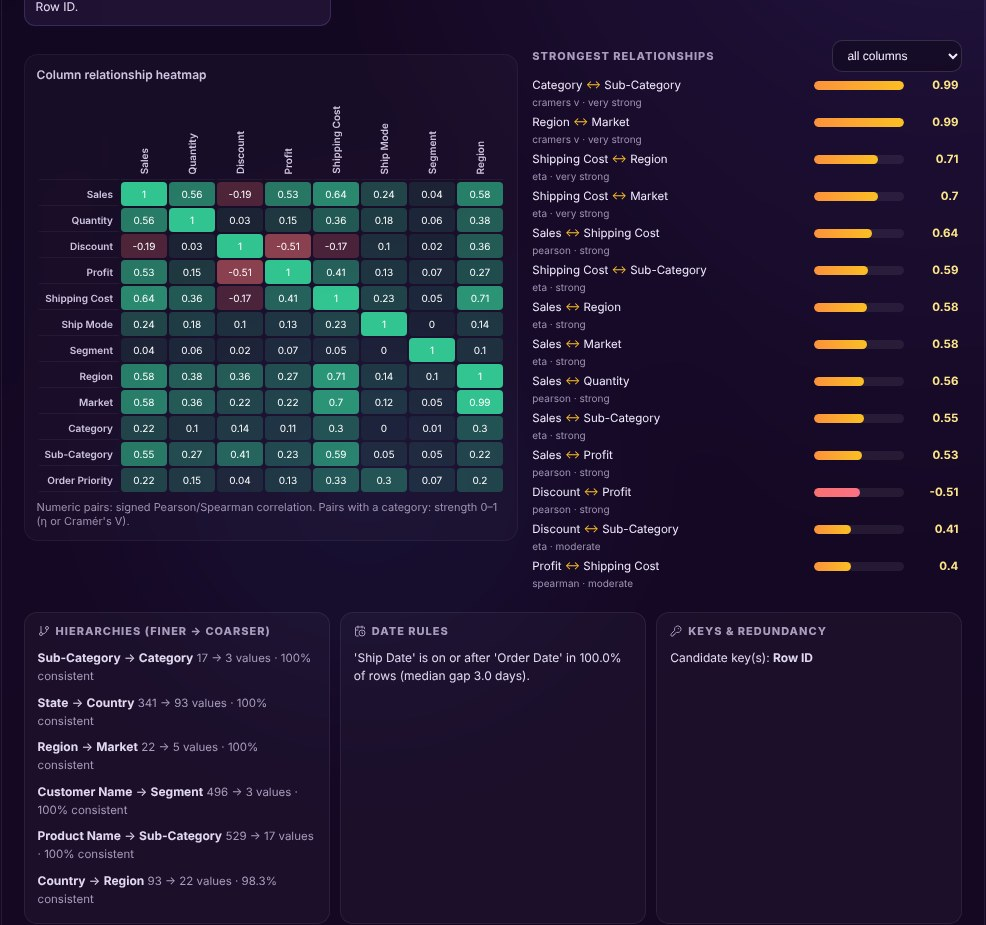
\includegraphics[width=\columnwidth]{figures/ui_relationships.jpg}
\caption{Relationships tab on Global Superstore: signed association heatmap, ranked pairs and detected hierarchies (Sub-Category$\to$Category, State$\to$Country, Region$\to$Market).}
\label{fig:rel}
\end{figure}

\subsection{Explainable AutoML}
Five regressors or classifiers (linear/logistic, decision tree, random forest, gradient boosting, XGBoost) are trained in preprocessing pipelines (imputation, scaling, one-hot encoding; identifiers, text and dates excluded). Selection uses $K$-fold CV on the training split (5 folds, 3 above 3,000 rows); to avoid choosing a complex model because of fold noise we apply the one-standard-error rule~\cite{hastie2009}:
\begin{equation}
m^{*}=\arg\min_{m}\ \mathrm{complexity}(m)\ \ \text{s.t.}\ \ \bar{e}_m\le \bar{e}_{\mathrm{best}}+\sigma_{\mathrm{best}}/\sqrt{K}.
\end{equation}
The winner is tuned by randomised search and kept only if CV improves, then evaluated once on a 20\% hold-out against a mean/majority baseline, with a paired fold test against the runner-up, a learning curve, a time-ordered 80/20 split when dates exist, and leakage screening (near-perfect correlation or single-feature AUC $\geq$0.99). Explanations are Shapley values on the \emph{raw} business columns, estimated by antithetic permutation sampling~\cite{strumbelj2014,lundberg2017}: ordering $\pi_k$ is paired with background row $b_k$ and
\begin{equation}
\phi_j(x)=\tfrac{1}{K}\textstyle\sum_{k}\big[f(z_{\pi_k,\le j})-f(z_{\pi_k,<j})\big],; f(x)=\phi_0+\textstyle\sum_j\phi_j,
\end{equation}
so additivity is exact (gap $<10^{-14}$ in our tests; error $<10^{-8}$ against closed-form Shapley values of a linear model). The UI shows global mean $|\phi|$ with direction and a per-prediction waterfall.

\subsection{Forecasting and decision intelligence}
Forecasts compare naive, seasonal-naive, moving-average, trend+season, ridge-autoregressive, random-forest and boosting lag models, damped Holt--Winters ETS and AIC-selected ARIMA/SARIMA in a rolling-origin backtest~\cite{hyndman2021}; sparse daily series are coarsened automatically, intervals (80/95\%) widen with the horizon from step-ahead backtest errors, and skill against the best baseline is always reported. \emph{explain\_change} decomposes a KPI change between two periods exactly over the groups $g$ of each dimension: $\Delta=\sum_g(M_{gB}-M_{gA})$ for sums, and $\Delta\bar{m}=\sum_g(w_{gB}-w_{gA})\bar m_{gA}+\sum_g w_{gB}(\bar m_{gB}-\bar m_{gA})$ (mix vs rate) for means; the dimension with the most concentrated contributions is reported with a waterfall. \emph{segment\_records} runs K-means with $k$ chosen by silhouette. A Business Analyst agent turns verified results into findings with a suggested action, evidence and, where arithmetic supports it, an illustrative impact (e.g.\ profit gained if low-margin groups reached the median margin), always labelled non-causal.

\subsection{Multi-agent reports and engineering}
For a business function, a Data Analyst agent (quality, relationships), a Business Analyst agent (function-specific KPIs, dimensions ranked by association with the outcome, comparisons, margins, trend, root cause), an ML agent (driver model with SHAP, segments, anomalies, forecast) and a Report agent assemble an executive summary, KPI cards, sections and ranked recommendations. Agents can only call validated tools; each call is logged in an agent trace shown in the UI and the PDF/Excel export. The Flask API adds SQLite persistence of datasets and conversations (restored after restart), optional authentication with owner-scoped sessions, rate limiting, background report jobs, metrics and a Docker image.

\begin{figure}[t]
\centering
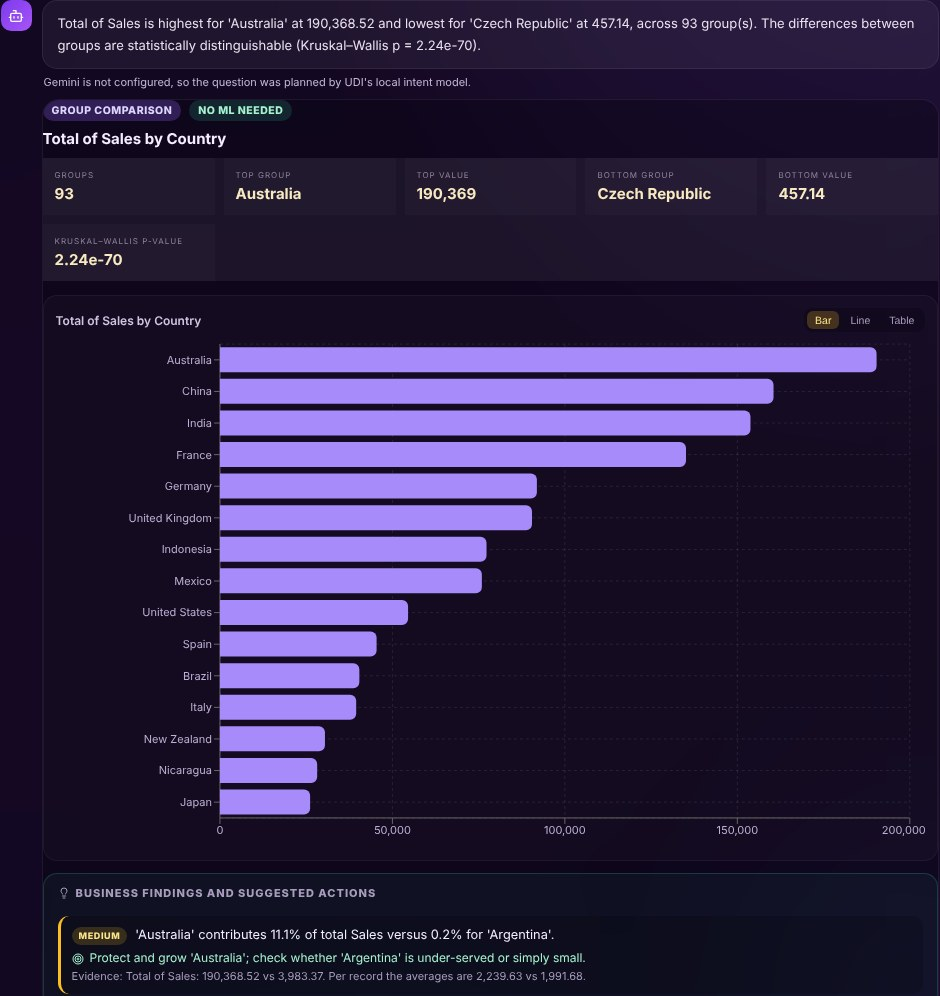
\includegraphics[width=\columnwidth]{figures/ui_answer.jpg}
\caption{Answer to ``Which country generated the most sales?'' on Global Superstore: planned locally, validated, computed in pandas, with a switchable chart and a business finding.}
\label{fig:ui}
\end{figure}

\section{Data and Experimental Setup}
\textbf{Datasets.} Four public datasets (Table~\ref{tab:data}) are bundled unchanged: a 1,000-order Global Superstore extract (sales, with countries, dates and missing postal codes), IBM HR Attrition (HR; itself simulated by IBM), IBM Telco Churn (marketing/customer; blank \texttt{TotalCharges}) and UCI Bank Marketing~\cite{moro2014} (41,188 calls). The seven 900-row generated Phase~1 datasets are reported separately.

\textbf{Benchmark.} We wrote 104 natural-language questions over six datasets (25 Superstore, 20 HR, 18 Telco, 15 Bank, 14 Company, 12 Hospital) covering all 18 operations, including 11 that must be refused (missing variable, unsupported request, no date column). Questions were phrased independently of the training templates, frozen, and run once through the full API; gold labels give the operation, target, grouping and filters, and 29 closed-form questions have an independent pandas oracle. We report the first run and, separately, a re-run after fixing the general defects it exposed (so the second number is no longer strictly held-out).

\textbf{Robustness.} Into IBM HR and Telco we injected 10\% missing values in two numeric columns, 2\% gross outliers, 1\% impossible negatives, 5\% case/spacing label variants and 3\% duplicate rows (seed 7), and measured detection recall per defect, the quality score and the macro-F1 of the selected classifier on original, corrupted and auto-cleaned data. All experiments use seed 42 and run with \texttt{evaluation/run\_real\_datasets.py}.

\begin{table}[t]
\caption{Public datasets: profile and data intelligence}
\label{tab:data}
\centering\scriptsize
\setlength{\tabcolsep}{3pt}
\resizebox{\columnwidth}{!}{%
\begin{tabular}{lrrcrcl}
\toprule
Dataset & Rows & Cols & $Q$ (grade) & Issues & Strong pairs & Structure found\\
\midrule
Global Superstore & 1,000 & 24 & 87.2 (B) & 3 & 12 & 6 hierarchies, ship$\geq$order\\
IBM HR Attrition & 1,470 & 35 & 100 (A) & 5 & 15 & key, 3 constant cols\\
IBM Telco Churn & 7,043 & 21 & 100 (A) & 1 & 37 & key, 11 blanks\\
UCI Bank Mkt. & 41,188 & 21 & 99.8 (A) & 3 & 20 & macro-indicator block\\
\bottomrule
\end{tabular}}
\end{table}

\section{Results}
\subsection{Question routing and numerical correctness}
Table~\ref{tab:bench} summarises the benchmark with the offline planner (median latency 0.02\,s per question excluding model training). On the frozen first run, intent accuracy was 97.1\%, numerical correctness 89.7\% and end-to-end correctness 88.5\%; 10 of 11 invalid requests were refused. Failures were concentrated in column linking: an outcome named \texttt{y} (``subscription rate''), ``campaign contacts by month'' grouping by \texttt{contact}, and a scenario verb attached to the wrong column. Fixing these general rules (dimensions are the columns after ``by''; a dataset's single outcome is the default classification target; change verbs must be adjacent to their column) raised end-to-end correctness to 96.2\%. The four remaining failures involve vocabulary absent from the schema (``how long do customers stay'', ``bed occupancy'', ``doctors on duty'') and one misrouted median question. Every numeric answer that was produced matched its oracle except where the wrong grouping had been planned; no answer contained a number not computed from the data.

\begin{table}[t]
\caption{Held-out NL benchmark (104 questions, 6 datasets, local planner)}
\label{tab:bench}
\centering\scriptsize
\begin{tabular}{lcc}
\toprule
Metric & Run 1 (frozen) & Run 2 (after fixes)\\
\midrule
Intent (operation) accuracy & 97.1\% (101/104) & 98.1\% (102/104)\\
Column mapping (target, group) & 85.3\% (64/75) & 96.0\% (72/75)\\
Filter extraction & 100\% (5/5) & 100\% (5/5)\\
Invalid-request rejection & 90.9\% (10/11) & 90.9\% (10/11)\\
Numerical correctness vs oracle & 89.7\% (26/29) & 96.6\% (28/29)\\
Answerable questions answered & 97.8\% (91/93) & 98.9\% (92/93)\\
\textbf{End-to-end pass} & \textbf{88.5\% (92/104)} & \textbf{96.2\% (100/104)}\\
\bottomrule
\end{tabular}
\end{table}

\subsection{AutoML and explanations on public data}
Table~\ref{tab:ml} reports the selected model per dataset; Fig.~\ref{fig:rel} shows the relationship view used to interpret them. All models beat their baselines on threshold-free metrics; accuracy alone would be misleading on imbalanced HR (selected 0.861 vs majority 0.840), which is why UDI reports macro-F1, ROC-AUC and PR-AUC. On Superstore, gradient boosting had the lowest CV RMSE (387.7) but random forest (395.7) lay within one standard error (23.6) and was chosen; tuning then lowered its 3-fold RMSE from 408.4 to 402.0. The time-ordered check on Superstore (R$^2$ 0.55 vs 0.71 random split) flags temporal drift that a random split hides. SHAP drivers are business-plausible: OverTime, MonthlyIncome and Age for attrition; Contract, InternetService and tenure for churn; call duration and macro indicators for subscription (duration is only known after a call, so it must be excluded when scoring clients before a call).

\begin{table*}[t]
\caption{Selected models on public data (CV on the training split; metrics on the untouched 20\% hold-out; macro-averaged F1)}
\label{tab:ml}
\centering\scriptsize
\setlength{\tabcolsep}{4pt}
\resizebox{\textwidth}{!}{%
\begin{tabular}{llcllcl}
\toprule
Dataset / target & Selected model & CV score (mean $\pm$ sd) & Held-out metrics & Baseline & Time-ordered check & Top SHAP drivers (share of mean $|\phi|$)\\
\midrule
Superstore / Profit & Random Forest (1-SE rule, tuned) & RMSE 396 $\pm$ 43 & R$^2$ 0.707, RMSE 290, MAE 214 & RMSE 536 & R$^2$ 0.554 & Discount 45\%, Sales 40\%, Shipping Cost 4\%\\
HR / Attrition & XGBoost & F1 0.718 $\pm$ 0.042 & F1 0.636, ROC-AUC 0.796, PR-AUC 0.504 & Acc. 0.840 & -- & OverTime 13\%, MonthlyIncome 8\%, Age 7\%\\
Telco / Churn & Random Forest & F1 0.734 $\pm$ 0.012 & F1 0.728, ROC-AUC 0.834, PR-AUC 0.640 & Acc. 0.735 & -- & Contract 19\%, InternetService 14\%, tenure 12\%\\
Bank / y & Random Forest & F1 0.782 $\pm$ 0.011 & F1 0.793, ROC-AUC 0.944, PR-AUC 0.661 & Acc. 0.888 & -- & duration 34\%, emp.var.rate 12\%, nr.employed 10\%\\
\bottomrule
\end{tabular}}
\end{table*}

\subsection{Data quality, forecasting and decision support}
The quality engine recovered 100\% of every injected defect type on both datasets (HR: 294 missing cells, 29 outliers, 14 negatives, 73 label variants, 44 duplicates; Telco five times larger). The score fell from 100 to 92.3 (HR) and 92.0 (Telco) and returned to 99.9 and 99.8 after auto-cleaning. Macro-F1 moved little (HR 0.636/0.618/0.647; Telco 0.729/0.732/0.725 for original/corrupted/cleaned), showing that the tree ensembles were robust to these defects and that the main value of cleaning here is correct descriptive statistics and group counts, not model accuracy. Fig.~\ref{fig:recall} summarises detection recall. The defects were gross by design, so recall on subtle real-world errors will be lower. For monthly Superstore sales, AIC-selected ARIMA won the backtest (RMSE 13,836, MAPE 24.1\%), 13.1\% better than the best baseline (moving average). In reports the agents surfaced decision-relevant gaps, e.g.\ attrition of 39.8\% for Sales Representatives versus 2.5\% for Research Directors, and churn of 42.7\% on month-to-month contracts versus 2.8\% on two-year contracts, each with the evidence and a non-causal illustrative impact.

\begin{figure}[t]
\centering
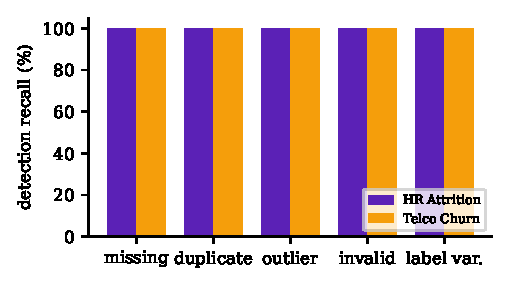
\includegraphics[width=0.92\columnwidth]{figures/fig_quality_recall.pdf}
\caption{Detection recall of the data-quality engine for five injected defect types.}
\label{fig:recall}
\end{figure}

\subsection{Generated reference domains and software verification}
On the seven generated datasets the dynamic engine reproduced Phase~1 behaviour (regression R$^2$ 0.28--0.90, classification macro-F1 0.72--1.00); perfect scores arise because the generated risk labels are deterministic functions of other columns, so these results are not evidence of real-world performance. The test suite now contains 168 executed tests (Phase~1 had 112 defined functions, 141 executed parametrised cases): all pass, including source scans for \texttt{exec}/\texttt{eval}, persistence across restarts, owner-scoped access, rate limiting and PDF/Excel export. The React production build was verified, and all six UI tabs were exercised in a headless browser.

\section{Discussion}
\textbf{Business value.} UDI moves from ``what happened'' to ``where and why it happened, and what to look at next'': the relationship map explains the schema, the quality score states how far the data can be trusted, SHAP and root-cause waterfalls justify each finding, and function-specific reports package them for marketing, HR or operations managers. The offline planner matters in practice: organisations that cannot send schemas to an external API still get a working assistant with the same validation guarantees.

\textbf{Limitations and threats to validity.} The benchmark was written by the project team and is small; it measures our planner on our phrasing and is not a user study, and the Gemini-mode benchmark (provided as a script) was not executed for this report because no API key was available in the evaluation environment. Run~2 is optimistic because fixes were informed by Run~1. The local planner relies on column names and a curated synonym list, so cryptic names (e.g.\ \texttt{y}) or vocabulary outside the schema fail. Analyses are associational: SHAP describes the model, root-cause decomposition shows where a change occurred, and impact estimates hold volumes constant. UDI handles one flat table per session.

\section{Conclusion}
UDI~2.0 shows that a conversational analyst can be both broad and verifiable: 18 validated operations, a relationship map, quality scoring with auditable cleaning, explainable AutoML, statistical forecasting, root-cause analysis and multi-agent reports, with no number ever produced by a language model. Future work: a user study with managers, the Gemini-mode benchmark, multi-table joins, conformal prediction intervals and causal uplift estimation for recommendations.

\section{Reproducibility}
Code, the four public datasets, the generated datasets, the benchmark, raw logs and figures are at \url{https://github.com/SamarthKamat/AMLBT_PROJECT}. Run \texttt{run\_windows.bat} or \texttt{run\_unix.sh} (Python 3.11+, Node 18+), or \texttt{docker compose up}; then \texttt{pytest}, \texttt{evaluation/run\_benchmark.py --planner local} and \texttt{evaluation/run\_real\_datasets.py} reproduce Tables~\ref{tab:bench}--\ref{tab:ml} (seed 42; package versions pinned in \texttt{requirements.txt} and \texttt{package-lock.json}). Gemini is optional; its outputs may vary between runs.

\subsection{AI Use Declaration}
\emph{Runtime:} Google Gemini is an optional component of UDI used only to plan questions and word verified results. \emph{Development:} in Phase~1, ChatGPT (OpenAI) was used for code assistance and, after the first review, to produce a design review that suggested the Phase~2 modules. In Phase~2, Claude Code (Anthropic) was used to implement and refactor backend and frontend code, write the tests, benchmark questions and evaluation scripts, run the experiments, and draft this manuscript and the documentation from the Phase~1 paper and the review feedback. The authors defined the requirements and scope, reviewed and ran the system, checked the reported results against the logs in the repository, and take responsibility for the content and conclusions.

\section*{Acknowledgment}
The authors thank Prof.\ Suman Sanyal, Course Coordinator, for guidance and feedback.

\footnotesize
\begin{thebibliography}{99}
\setlength{\itemsep}{0pt}
\bibitem{hong2024} Z. Hong \emph{et al.}, ``Next-generation database interfaces: A survey of LLM-based text-to-SQL,'' arXiv:2406.08426, 2024.
\bibitem{tang2025} Z. Tang \emph{et al.}, ``LLM/Agent-as-Data-Analyst: A survey,'' arXiv:2509.23988, 2025.
\bibitem{sun2024} M. Sun \emph{et al.}, ``A survey on large language model-based agents for statistics and data science,'' arXiv:2412.14222, 2024.
\bibitem{zhang2023} W. Zhang, Y. Shen, W. Lu, and Y. Zhuang, ``Data-Copilot: Bridging billions of data and humans with autonomous workflow,'' arXiv:2306.07209, 2023.
\bibitem{lambda2024} M. Sun \emph{et al.}, ``LAMBDA: A large model based data agent,'' arXiv:2407.17535, 2024.
\bibitem{hong2024di} S. Hong \emph{et al.}, ``Data Interpreter: An LLM agent for data science,'' arXiv:2402.18679, 2024.
\bibitem{zhangautoml} S. Zhang \emph{et al.}, ``AutoML-GPT: Automatic machine learning with GPT,'' arXiv:2305.02499, 2023.
\bibitem{saha2024} D. Saha, K. Singh, M. Mahato, and J. Nabi, ``Analytics Graph Query Solver (AGQS),'' in \emph{Proc. ICON}, 2024, pp. 537--553.
\bibitem{sun2025agentic} J. Sun \emph{et al.}, ``AgenticData: An agentic data analytics system for heterogeneous data,'' arXiv, 2025.
\bibitem{liao2026} Y. Liao \emph{et al.}, ``SageCopilot: An LLM-empowered autonomous agent for data science as a service,'' \emph{IEEE Trans. Services Comput.}, 2026.
\bibitem{schick2023} T. Schick \emph{et al.}, ``Toolformer: Language models can teach themselves to use tools,'' arXiv:2302.04761, 2023.
\bibitem{yao2022} S. Yao \emph{et al.}, ``ReAct: Synergizing reasoning and acting in language models,'' arXiv:2210.03629, 2022.
\bibitem{lundberg2017} S. M. Lundberg and S.-I. Lee, ``A unified approach to interpreting model predictions,'' in \emph{Proc. NeurIPS}, 2017, pp. 4765--4774.
\bibitem{strumbelj2014} E. \v{S}trumbelj and I. Kononenko, ``Explaining prediction models and individual predictions with feature contributions,'' \emph{Knowl. Inf. Syst.}, vol. 41, no. 3, pp. 647--665, 2014.
\bibitem{hastie2009} T. Hastie, R. Tibshirani, and J. Friedman, \emph{The Elements of Statistical Learning}, 2nd ed. New York, NY, USA: Springer, 2009.
\bibitem{liu2008} F. T. Liu, K. M. Ting, and Z.-H. Zhou, ``Isolation forest,'' in \emph{Proc. IEEE ICDM}, 2008, pp. 413--422.
\bibitem{iglewicz1993} B. Iglewicz and D. C. Hoaglin, \emph{How to Detect and Handle Outliers}. Milwaukee, WI, USA: ASQC Quality Press, 1993.
\bibitem{bergsma2013} W. Bergsma, ``A bias-correction for Cram\'er's V and Tschuprow's T,'' \emph{J. Korean Stat. Soc.}, vol. 42, no. 3, pp. 323--328, 2013.
\bibitem{wang1996} R. Y. Wang and D. M. Strong, ``Beyond accuracy: What data quality means to data consumers,'' \emph{J. Manage. Inf. Syst.}, vol. 12, no. 4, pp. 5--33, 1996.
\bibitem{hyndman2021} R. J. Hyndman and G. Athanasopoulos, \emph{Forecasting: Principles and Practice}, 3rd ed. Melbourne, Australia: OTexts, 2021.
\bibitem{moro2014} S. Moro, P. Cortez, and P. Rita, ``A data-driven approach to predict the success of bank telemarketing,'' \emph{Decis. Support Syst.}, vol. 62, pp. 22--31, 2014.
\end{thebibliography}
\end{document}
